\documentclass[11pt]{article}
\usepackage[a4paper,includeheadfoot,margin=2.54cm]{geometry}
\usepackage{parskip}

% fonte adotada
\usepackage{mathpazo}
\usepackage{domitian}
\usepackage[T1]{fontenc}
\let\oldstylenums\oldstyle

\usepackage{hyperref}
\usepackage{graphicx}

\begin{document}

\underline{\textbf{Atividade 19 - Diagrama de Loop Causal}}\par
\textbf{Sistemas de Informação}\\
\textbf{Instituto Federal do Espírito Santo}\\
Campus Serra - Espírito Santo\par
\textbf{Teoria Geral de Sistemas}\\
Prof. Dr. Rodrigo Fernandes Calhau\par
Anderson A. Fraga (20222BSI0482)\\
\texttt{aafrg@tuta.io}\\  %\texttt formats the text to a typewriter style font

\begin{enumerate}
    \item Realizar o diagrama de loop causal (mapa sistêmico) relativo ao estudo de caso 7 e 8 na página 194 a 196 do livro \href{https://drive.google.com/file/d/1eJU2qK8IzC-S8jRKQuHrIgED1tEvzGOq/view}{Desvendando Sistemas}.

        \textbf{Estudo de caso 7}\par
        \begin{figure}[!h]
            \centering
            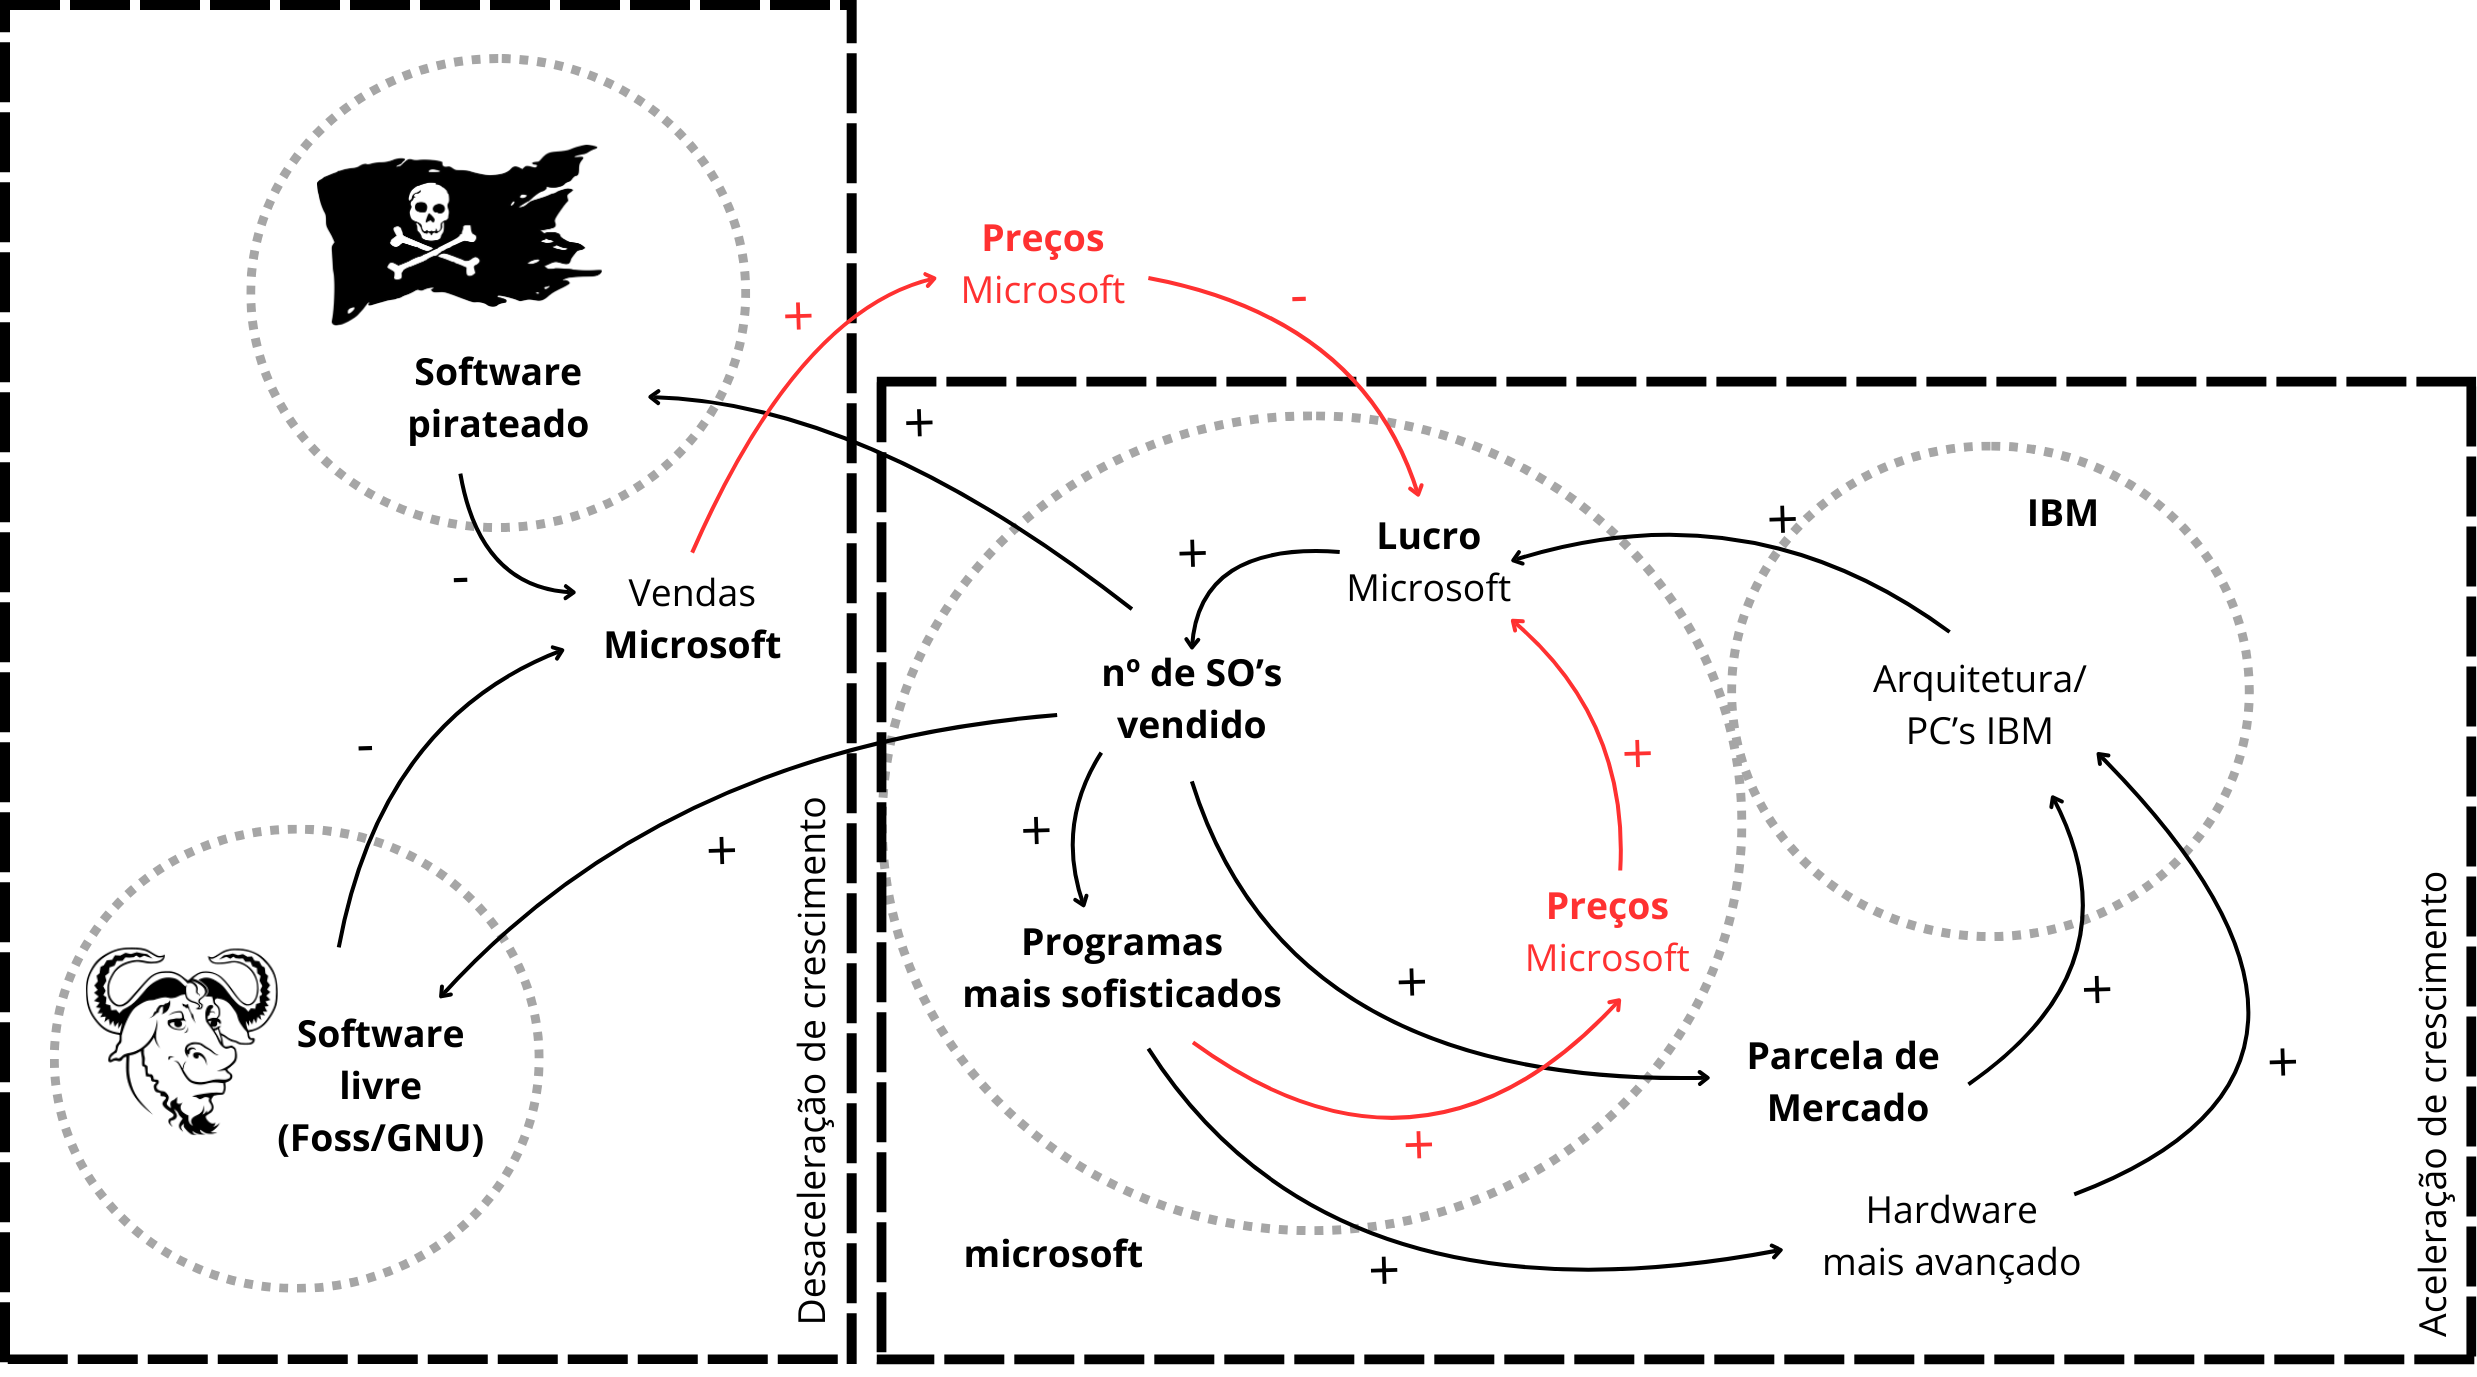
\includegraphics[width=0.90\linewidth]{img/diagrama1-ec7.png}
        \end{figure}
\pagebreak
        \textbf{Estudo de caso 8}\par
        \begin{figure}[!ht]
            \centering
            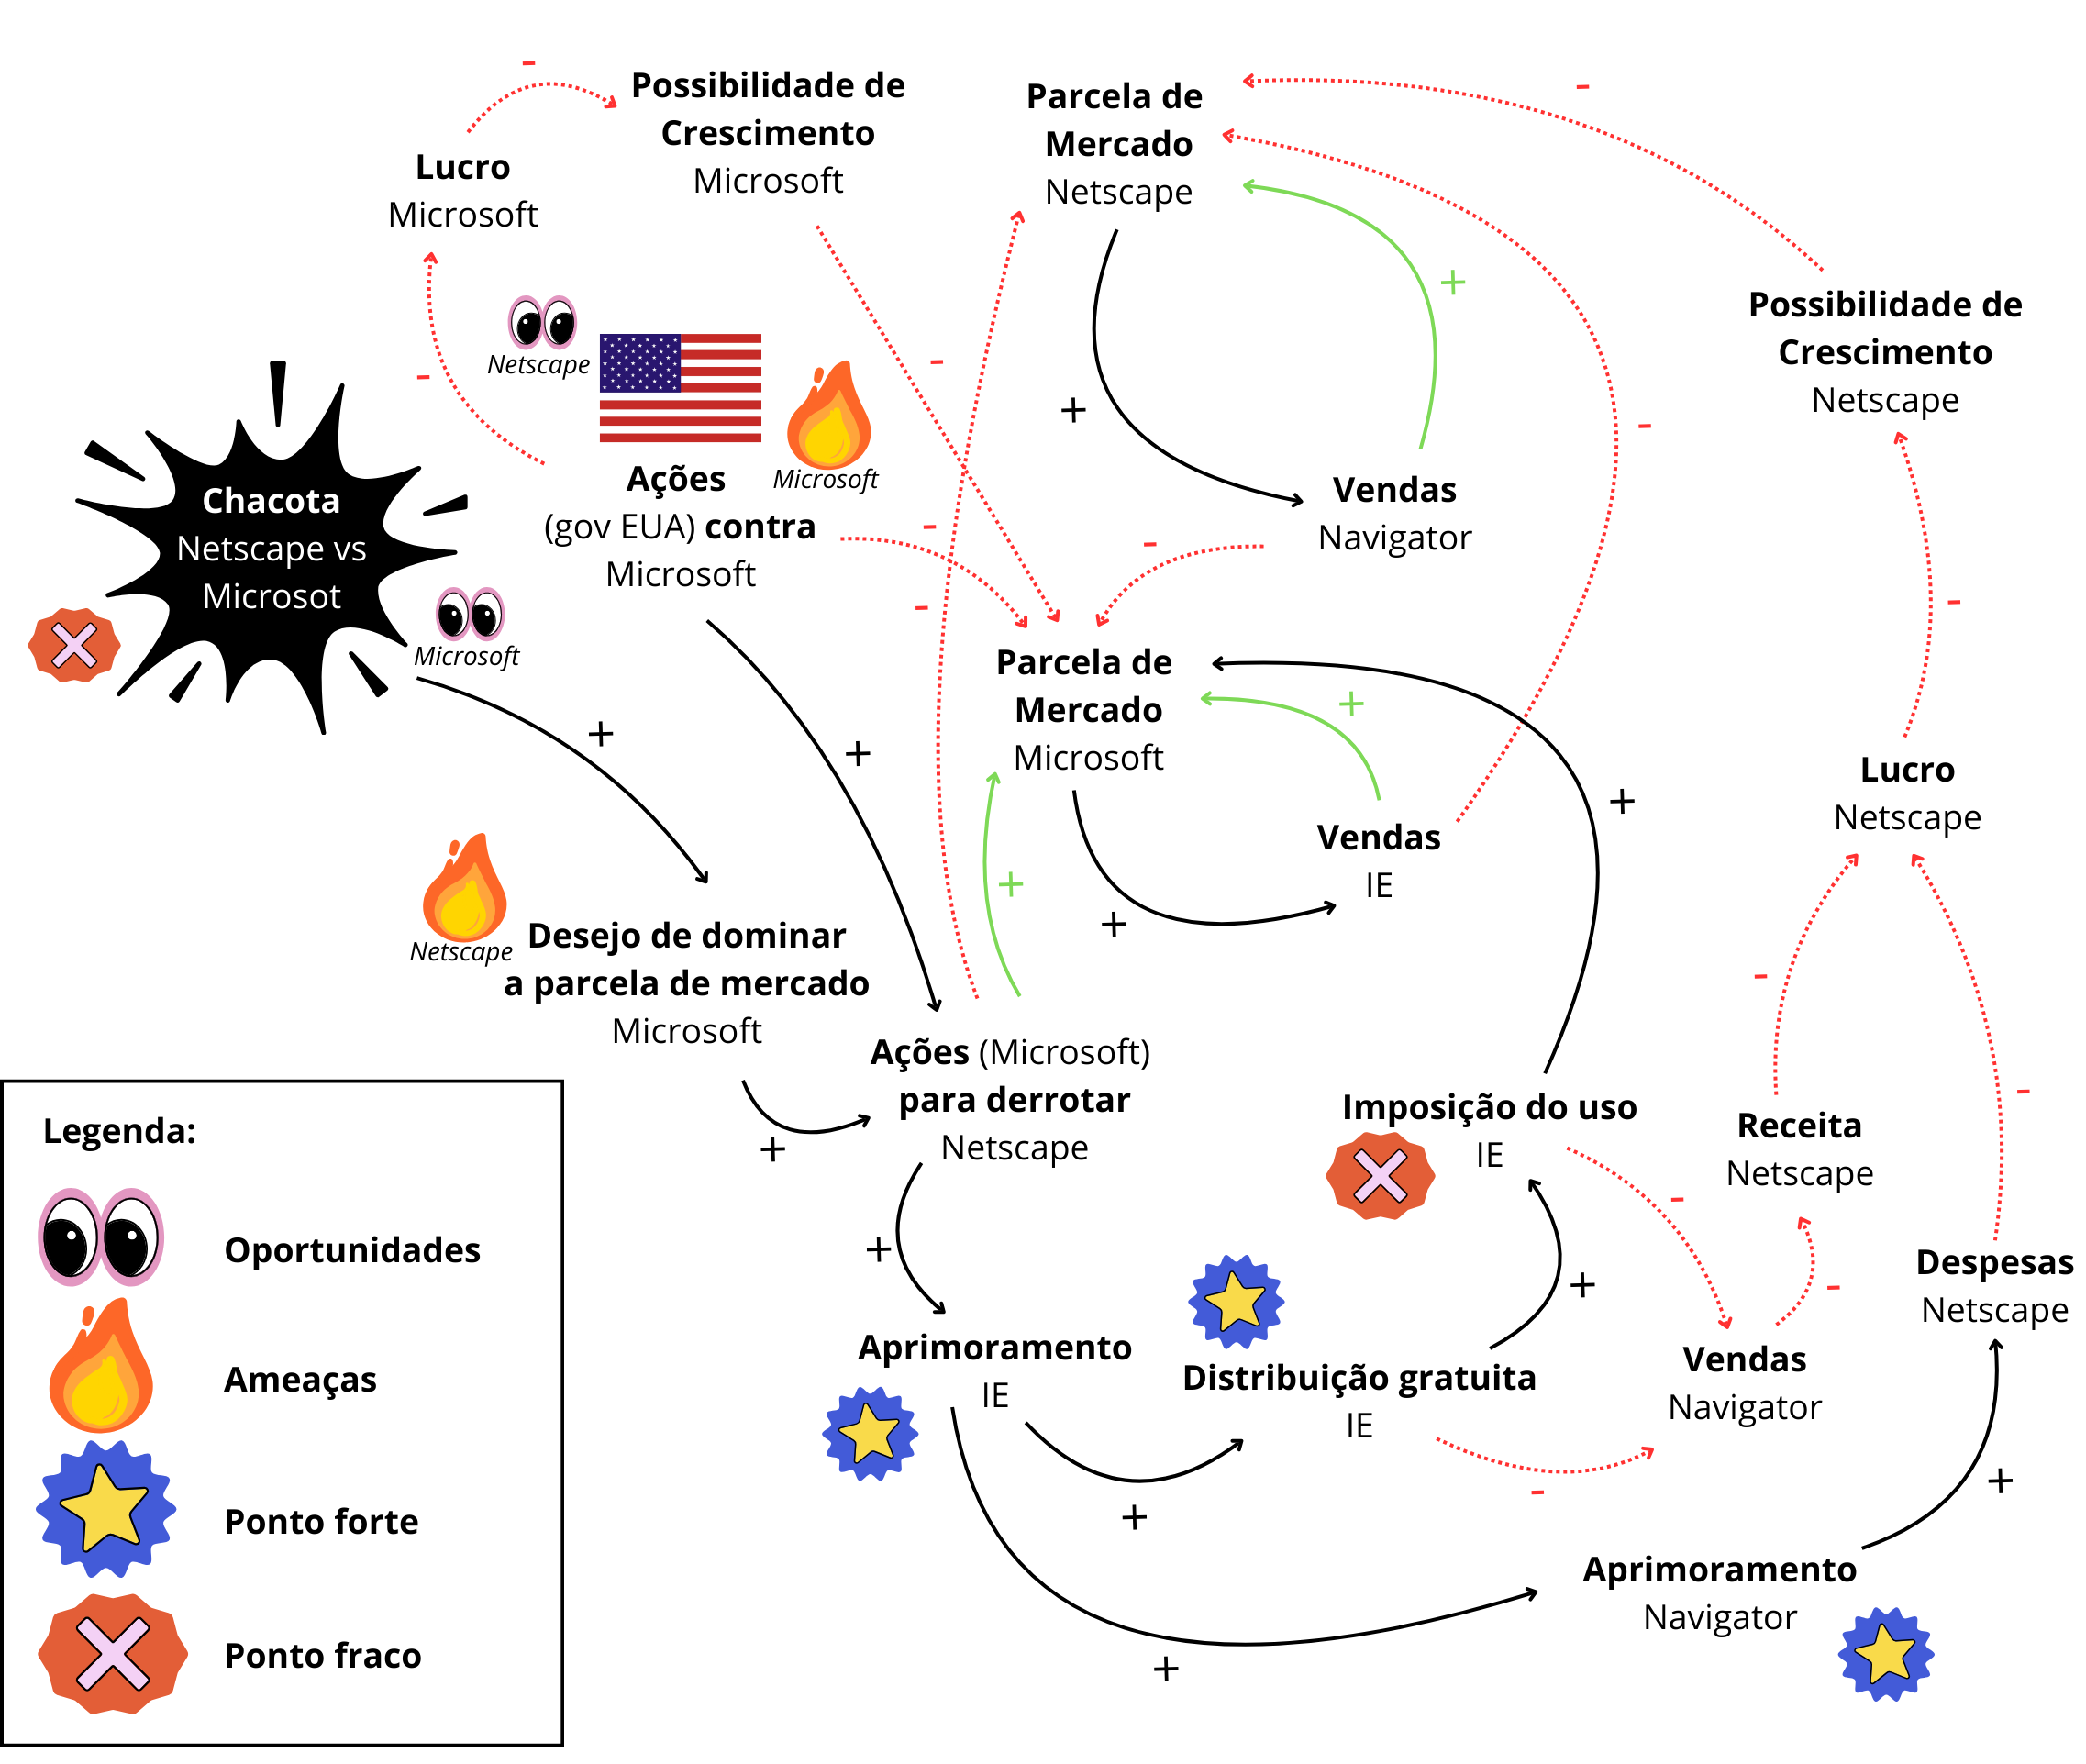
\includegraphics[width=0.95\linewidth]{img/diagrama2-ec8.png}
        \end{figure}

\end{enumerate}

\end{document}
